% % % % % % % % % % % % % % % % % % % % % % % % % % % % % % % % % %
%  Devolutiva — Fase 1: Imersão
%  Disciplina: Design Thinking (DE_233) — ETE Cícero Dias
%  Profa. Samara Silva  ·  Recife, 28 de junho de 2026
% % % % % % % % % % % % % % % % % % % % % % % % % % % % % % % % % %

\documentclass[
  sigconf,
  nonacm, % Remove o rodapé da ACM
  language=portuguese
]{acmart}

% ── Desliga rodapé ACM ──────────────────────────────────────
\settopmatter{printacmref=false}
\setcopyright{none}
\acmYear{2026}
\let\balance\relax

% ── Mata a página temporária da ACM (compilação única via API) ──
\makeatletter
\def\acm@addtemp@page{}
\makeatother

% ── Pacotes ─────────────────────────────────────────────────
\usepackage[portuguese]{babel}
\usepackage{microtype}
\usepackage{booktabs}
\usepackage{tabularx}
\usepackage{array}
\usepackage{colortbl}
\usepackage[dvipsnames,table]{xcolor}
\usepackage[inline]{enumitem}
\usepackage{graphicx}
\usepackage{adjustbox}
\usepackage{fancyhdr}
\usepackage{eso-pic} % Para a capa preencher toda a página sem gerar páginas em branco

% ── Ajuste contra quebras de texto ruins (Textos Cortados) ──
\tolerance=1000
\emergencystretch=1.5em

% ── Cores ───────────────────────────────────────────────────
\definecolor{cgood}{HTML}{1E6B3A}
\definecolor{cwarn}{HTML}{8B4500}
\definecolor{cred}{HTML}{C0392B}
\definecolor{cmuted}{HTML}{666666}
\definecolor{crow}{HTML}{F2EFEB}

% ── Colunas customizadas para tabela ────────────────────────
\newcolumntype{L}[1]{>{\raggedright\arraybackslash}p{#1}}
\newcolumntype{C}[1]{>{\centering\arraybackslash}p{#1}}

% ── Comando nota destacada ───────────────────────────────────
\newcommand{\notadestaque}[2]{%
  \noindent\textbf{Nota:}\enspace%
  {\large\bfseries\color{cred}#1\,/\,#2\,pts}%
}

% ── Comando label de status ──────────────────────────────────
\newcommand{\statusok}[1]{{\small\bfseries\color{cgood}#1}}
\newcommand{\statuswarn}[1]{{\small\bfseries\color{cwarn}#1}}

% ── Renomeações PT-BR ────────────────────────────────────────
\AtBeginDocument{%
  \renewcommand{\abstractname}{Resumo}
  \renewcommand{\figurename}{Figura}
  \renewcommand{\tablename}{Tabela}
}

% ────────────────────────────────────────────────────────────
\begin{document}

% ── CAPA ────────────────────────────────────────────────────
\thispagestyle{empty}
\AddToShipoutPictureBG*{%
  \AtPageLowerLeft{%
    \IfFileExists{capa.png}{%
      
\includegraphics[width=\paperwidth,height=\paperheight]{capa.png}%
    }{%
      \IfFileExists{../../capa.png}{%
        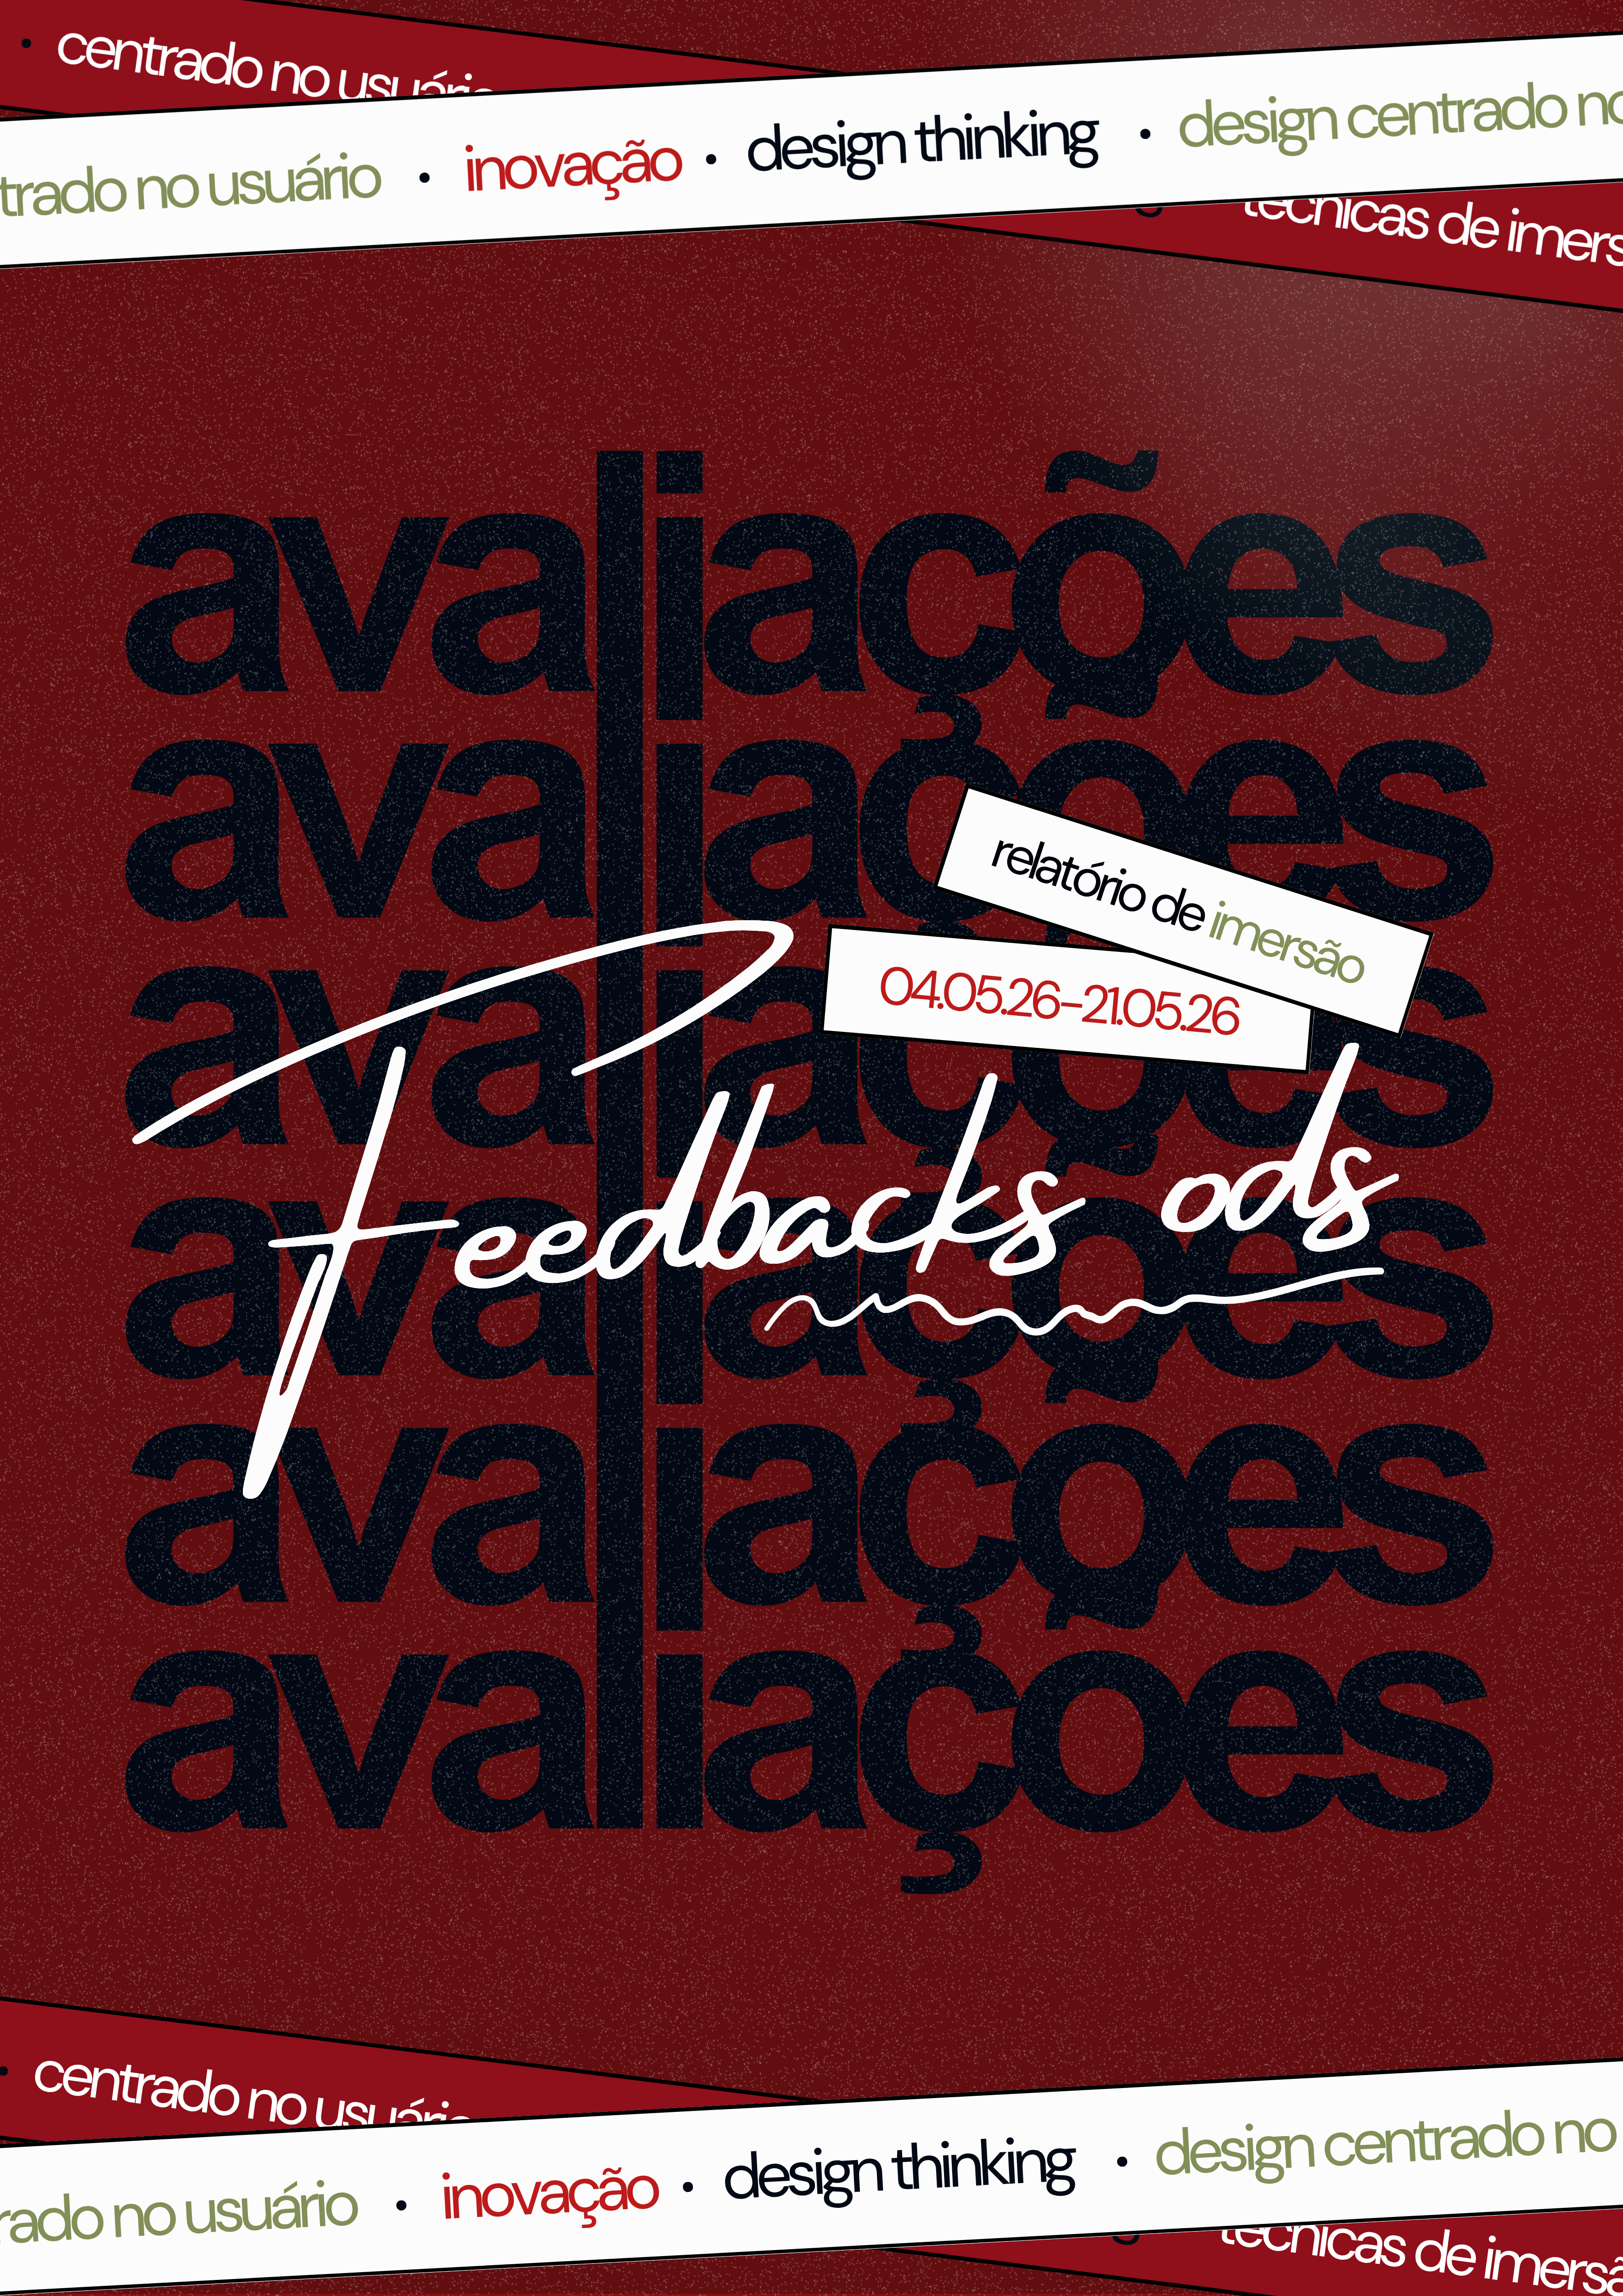
\includegraphics[width=\paperwidth,height=\paperheight]{../../capa.png}%
      }{%
        \parbox[b][\paperheight]{\paperwidth}{%
          \vspace*{10cm}\begin{center}{\large\color{gray}[capa.png não encontrada]}\end{center}%
        }%
      }%
    }%
  }%
}
\mbox{} % Caixa vazia para garantir que a página da capa seja gerada e preenchida
\clearpage

% ── CONFIGURAÇÃO DE PÁGINA PÓS-CAPA ─────────────────────────
\setcounter{page}{1}
\pagestyle{fancy}
\fancyhf{}
\renewcommand{\headrulewidth}{0pt}
\fancyfoot[C]{\thepage}
\setlength{\headsep}{0.8cm} % Distancia o cabeçalho do conteúdo das colunas

% ── METADADOS ────────────────────────────────────────────────
\title{Feedback Avaliativo de Projeto: Design Thinking --- Avaliação Completa}

\author{Profa.\ Samara Silva}
\authornote{Grupo: \textbf{Grupo 02 - Moda Sustentável} \textperiodcentered\ Per\'{i}odo: 22 de maio de 2026 \textperiodcentered\ Avaliado em: 28 de junho de 2026.}
\email{samarasilvia.educa@gmail.com}
\affiliation{%
  \institution{ETE C\'{i}cero Dias}
  \department{M\'{o}dulo 1 --- Turma A · 2026.1}
  \city{Recife}
  \state{Pernambuco}
  \country{Brasil}
}

\author{Grupo 02 - Moda Sustentável}
\affiliation{%
  \institution{ETE C\'{i}cero Dias}
  \department{Turma --- Turma A · 2026.1}
  \city{Recife}
  \state{Pernambuco}
  \country{Brasil}
}
\maketitle

\vspace{1em}
\section{Avaliação — Design Thinking}

\notadestaque{9,27}{11,00}

A seguir o detalhamento por fase da disciplina.

\subsection{Fase 1 — Imersão}

\notadestaque{2,47}{3,00}

\subsubsection*{Resumo dos Critérios}

\rowcolors{2}{crow}{white}
\begin{tabular}{@{} L{2.6cm} C{2.5cm} C{1.1cm} C{1.1cm} @{}}
\toprule
\textbf{Critério} & \textbf{Status} & \textbf{Nota} & \textbf{Máx.} \\
\midrule
Pesquisa Desk & \statusok{Completo} & \textbf{0,50} & 0,50 \\
Matriz de Alinhamento & \statusok{Completo} & \textbf{0,50} & 0,50 \\
Matriz CSD \& Perguntas de pesquisa & \statuswarn{Completo c/ ressalvas} & \textbf{0,42} & 0,50 \\
Pesquisa Primária & \statuswarn{Completo, mas inadequado} & \textbf{1,05} & 1,50 \\
\midrule
\textbf{Total} & & \textbf{\color{cred}2,47} & \textbf{3,00} \\
\bottomrule
\end{tabular}

\subsubsection*{Comentários}

\subsection{Pesquisa Desk}

\noindent\statusok{0,50\,/\,0,50 pts · Completo}

\begin{itemize}[leftmargin=14pt,itemsep=1pt,topsep=3pt,parsep=0pt]
  \item[\textcolor{cgood}{$\checkmark$}] {\small\textcolor{cgood}{Dados secundários relevantes e atuais sobre o ODS escolhido}}
  \item[\textcolor{cgood}{$\checkmark$}] {\small\textcolor{cgood}{Fontes confiáveis: ONU, IBGE, artigos acadêmicos ou jornalísticos}}
  \item[\textcolor{cgood}{$\checkmark$}] {\small\textcolor{cgood}{Contextualiza o problema com base factual}}
  \item[\textcolor{cgood}{$\checkmark$}] {\small\textcolor{cgood}{Conexão clara entre os dados e o problema}}
  \item[\textcolor{cgood}{$\checkmark$}] {\small\textcolor{cgood}{Coerência entre a CSD e o que foi pesquisado}}
  \item[\textcolor{cgood}{$\checkmark$}] {\small\textcolor{cgood}{Mínimo de 5 referências/links, esperado 8, ideal de 15 para cima}}
\end{itemize}

\subsection{Matriz de Alinhamento}

\noindent\statusok{0,50\,/\,0,50 pts · Completo}

\begin{itemize}[leftmargin=14pt,itemsep=1pt,topsep=3pt,parsep=0pt]
  \item[\textcolor{cgood}{$\checkmark$}] {\small\textcolor{cgood}{Identifica claramente quem é afetado pelo problema}}
  \item[\textcolor{cgood}{$\checkmark$}] {\small\textcolor{cgood}{Define o que o grupo pretende descobrir durante a imersão}}
  \item[\textcolor{cgood}{$\checkmark$}] {\small\textcolor{cgood}{As técnicas de imersão escolhidas são coerentes com os objetivos da pesquisa}}
  \item[\textcolor{cgood}{$\checkmark$}] {\small\textcolor{cgood}{Delimita adequadamente o que está dentro do escopo do projeto}}
  \item[\textcolor{cgood}{$\checkmark$}] {\small\textcolor{cgood}{Delimita adequadamente o que está fora do escopo do projeto}}
  \item[\textcolor{cgood}{$\checkmark$}] {\small\textcolor{cgood}{Apresenta uma hipótese inicial de solução relacionada ao problema investigado}}
  \item[\textcolor{cgood}{$\checkmark$}] {\small\textcolor{cgood}{Os resultados esperados da imersão são claros e coerentes com os objetivos da pesquisa}}
  \item[\textcolor{cgood}{$\checkmark$}] {\small\textcolor{cgood}{Há coerência entre os diferentes campos da matriz (problema, público, escopo, pesquisa e solução)}}
  \item[\textcolor{cgood}{$\checkmark$}] {\small\textcolor{cgood}{Preenchida com respostas, impressões ou perguntas reais do grupo sobre o problema}}
  \item[\textcolor{cgood}{$\checkmark$}] {\small\textcolor{cgood}{Linguagem clara e coerente, facilitando a compreensão das intenções do grupo}}
  \item[\textcolor{cgood}{$\checkmark$}] {\small\textcolor{cgood}{Serviu de base para planejar a pesquisa primária}}
\end{itemize}

\subsection{Matriz CSD \& Perguntas de pesquisa}

\noindent\statuswarn{0,42\,/\,0,50 pts · Completo c/ ressalvas}

\begin{itemize}[leftmargin=14pt,itemsep=1pt,topsep=3pt,parsep=0pt]
  \item[\textcolor{cgood}{$\checkmark$}] {\small\textcolor{cgood}{Os três quadrantes preenchidos: Certezas, Suposições, Dúvidas}}
  \item[\textcolor{cgood}{$\checkmark$}] {\small\textcolor{cgood}{Reflete o que o grupo sabe e precisa descobrir sobre o problema e seu contexto}}
  \item[\textcolor{cgood}{$\checkmark$}] {\small\textcolor{cgood}{Conteúdo específico do projeto — não genérico}}
  \item[\textcolor{cgood}{$\checkmark$}] {\small\textcolor{cgood}{Revela pensamento crítico}}
  \item[\textcolor{cgood}{$\checkmark$}] {\small\textcolor{cgood}{O quadrante de CERTEZAS expõe informações comprovadas ou confirmadas sobre o problema}}
  \item[\textcolor{cgood}{$\checkmark$}] {\small\textcolor{cgood}{Os itens do quadrante de CERTEZA estão relacionados diretamente ao contexto e ao público afetado}}
  \item[\textcolor{cgood}{$\checkmark$}] {\small\textcolor{cgood}{O quadrante de SUPOSIÇÕES expõe Informações que o grupo acha que são verdadeiras, mas ainda não comprovou}}
  \item[\textcolor{cgood}{$\checkmark$}] {\small\textcolor{cgood}{Os itens do quadrante de SUPOSIÇÃO demonstram reflexão sobre possíveis causas, comportamentos ou necessidades}}
  \item[\textcolor{cgood}{$\checkmark$}] {\small\textcolor{cgood}{O quadrante de DÚVIDAS expõem perguntas que o grupo precisa responder na pesquisa ou imersão como um todo}}
  \item[\textcolor{cgood}{$\checkmark$}] {\small\textcolor{cgood}{Os itens do quadrante de DÚVIDAS representam lacunas reais de conhecimento}}
  \item[\textcolor{cgood}{$\checkmark$}] {\small\textcolor{cgood}{O conteúdo da matriz está focado no problema investigado e não apenas no tema ou na ODS}}
  \item[$\square$] {\small\textcolor{cmuted}{Perguntas de Pesquisas formuladas como objetivos que norteiam o projeto geral}}
  \item[$\square$] {\small\textcolor{cmuted}{Deve se ter um mínimo de 5 itens no quadrante de certezas, suposições e dúvidas}}
\end{itemize}

\subsection{Pesquisa Primária}

\noindent\statuswarn{1,05\,/\,1,50 pts · Completo, mas inadequado}

Embora tenham corrigido os dados permanentes são de acordo com o primeiro formulário feito tendo apenas 4 perguntas e 22 respostas, por isso não pontuaram 100\% nesse quesito. 

O único comentário que faço em relação ao registro na documentação é por quanto tempo ficou o formulário no ar ? Faltou essa informação, mas não afeta o desenvolvimento do projeto, por isso não despontuei.

Como também usaram de outra técnica de imersão, observação direta, ao invés de pontuar com "Faltou pouco", coloquei completo, mas não feito da melhor forma (inadequado), porque não prejudica muito o projeto de vocês, mas ainda prejudica, porque carece de dados que são importantes. O fato de saber se a maioria das pessoas que respondeu é jovem, adulto, ou maior e idade impacta na acessibilidade e usabilidade que o sistema de vocês terá.

\subsection{Fase 2 — Definição}

\notadestaque{2,85}{3,00}

\subsubsection*{Resumo dos Critérios}

\rowcolors{2}{crow}{white}
\begin{tabular}{@{} L{2.6cm} C{2.5cm} C{1.1cm} C{1.1cm} @{}}
\toprule
\textbf{Critério} & \textbf{Status} & \textbf{Nota} & \textbf{Máx.} \\
\midrule
Persona com Empatia Real & \statusok{Completo} & \textbf{0,50} & 0,50 \\
Mapa de Empatia como Ferramenta & \statusok{Completo} & \textbf{1,00} & 1,00 \\
Enunciado do Problema & \statuswarn{Completo c/ ressalvas} & \textbf{0,85} & 1,00 \\
Jornada do Usuário (ASTOIS) & \statusok{Completo} & \textbf{0,50} & 0,50 \\
\midrule
\textbf{Total} & & \textbf{\color{cred}2,85} & \textbf{3,00} \\
\bottomrule
\end{tabular}

\subsubsection*{Comentários}

\subsection{Persona com Empatia Real}

\noindent\statusok{0,50\,/\,0,50 pts · Completo}

\begin{itemize}[leftmargin=14pt,itemsep=1pt,topsep=3pt,parsep=0pt]
  \item[\textcolor{cgood}{$\checkmark$}] {\small\textcolor{cgood}{Nome próprio que humaniza o arquétipo}}
  \item[\textcolor{cgood}{$\checkmark$}] {\small\textcolor{cgood}{Representação visual coerente (foto/avatar)}}
  \item[\textcolor{cgood}{$\checkmark$}] {\small\textcolor{cgood}{Papel/arquétipo-síntese (o rótulo: ex: "Pequeno Comerciante")}}
  \item[\textcolor{cgood}{$\checkmark$}] {\small\textcolor{cgood}{Dados demográficos (idade, gênero, localização, escolaridade, ocupação, estado civil)}}
  \item[\textcolor{cgood}{$\checkmark$}] {\small\textcolor{cgood}{Contexto/bio que situa a vida da pessoa}}
  \item[\textcolor{cgood}{$\checkmark$}] {\small\textcolor{cgood}{Características de personalidade (traços comportamentais)}}
  \item[\textcolor{cgood}{$\checkmark$}] {\small\textcolor{cgood}{Motivação (o que move)}}
  \item[\textcolor{cgood}{$\checkmark$}] {\small\textcolor{cgood}{Objetivos/metas}}
  \item[\textcolor{cgood}{$\checkmark$}] {\small\textcolor{cgood}{Dores/frustrações}}
  \item[\textcolor{cgood}{$\checkmark$}] {\small\textcolor{cgood}{Citação-síntese que captura a essência}}
  \item[\textcolor{cgood}{$\checkmark$}] {\small\textcolor{cgood}{Ancoragem na imersão — a persona é síntese da pesquisa de campo, não invenção/suposição}}
  \item[\textcolor{cgood}{$\checkmark$}] {\small\textcolor{cgood}{Arquétipo comportamental, não estereótipo ou caricatura}}
  \item[\textcolor{cgood}{$\checkmark$}] {\small\textcolor{cgood}{Coerência interna — motivação → objetivos → dores se sustentam mutuamente}}
  \item[\textcolor{cgood}{$\checkmark$}] {\small\textcolor{cgood}{Conexão com o problema e o ODS do projeto}}
  \item[\textcolor{cgood}{$\checkmark$}] {\small\textcolor{cgood}{Especificidade — detalhes concretos que humanizam vs. genérico ("homem de 40 anos qualquer")}}
  \item[\textcolor{cgood}{$\checkmark$}] {\small\textcolor{cgood}{Define claramente as tarefas críticas que o usuário precisa executar}}
\end{itemize}

\subsection{Mapa de Empatia como Ferramenta}

\noindent\statusok{1,00\,/\,1,00 pts · Completo}

\begin{itemize}[leftmargin=14pt,itemsep=1pt,topsep=3pt,parsep=0pt]
  \item[\textcolor{cgood}{$\checkmark$}] {\small\textcolor{cgood}{Os 7 quadrantes foram preenchidos corretamente}}
  \item[\textcolor{cgood}{$\checkmark$}] {\small\textcolor{cgood}{Informa com QUEM está se demonstrando empatia}}
  \item[\textcolor{cgood}{$\checkmark$}] {\small\textcolor{cgood}{O que ele VÊ - Descreve o que o usuário enxerga no seu ambiente/contexto relacionado ao problema}}
  \item[\textcolor{cgood}{$\checkmark$}] {\small\textcolor{cgood}{O que o usuário DIZ (expressões, o que ele verbaliza)}}
  \item[\textcolor{cgood}{$\checkmark$}] {\small\textcolor{cgood}{O que ele FAZ (comportamentos observados no contexto do problema)}}
  \item[\textcolor{cgood}{$\checkmark$}] {\small\textcolor{cgood}{O que ele OUVE - Descreve o que o usuário escuta de pessoas e meios ao seu redor sobre o problema}}
  \item[\textcolor{cgood}{$\checkmark$}] {\small\textcolor{cgood}{O que ele PENSA (crenças, valores, como vê o mundo)}}
  \item[\textcolor{cgood}{$\checkmark$}] {\small\textcolor{cgood}{O que ele SENTE (emoções, medos, esperanças)}}
  \item[\textcolor{cgood}{$\checkmark$}] {\small\textcolor{cgood}{Dores (frustrações existenciais, medos profundos, obstáculos à vida)}}
  \item[\textcolor{cgood}{$\checkmark$}] {\small\textcolor{cgood}{Ganhos (aspirações, o que o faria feliz, sonhos)}}
  \item[$\square$] {\small\textcolor{cmuted}{Não há presença de itens inacabados ou derivados do template}}
\end{itemize}

\subsection{Enunciado do Problema}

\noindent\statuswarn{0,85\,/\,1,00 pts · Completo c/ ressalvas}

\begin{itemize}[leftmargin=14pt,itemsep=1pt,topsep=3pt,parsep=0pt]
  \item[\textcolor{cgood}{$\checkmark$}] {\small\textcolor{cgood}{Enunciado que resume o problema estudado}}
  \item[\textcolor{cgood}{$\checkmark$}] {\small\textcolor{cgood}{O problema é específico e decorre da pesquisa}}
  \item[\textcolor{cgood}{$\checkmark$}] {\small\textcolor{cgood}{Presença de afirmação diagnótica}}
  \item[\textcolor{cgood}{$\checkmark$}] {\small\textcolor{cgood}{Presença do público-alvo afetado}}
  \item[$\square$] {\small\textcolor{cmuted}{O público-alvo é contextual, observável e específico}}
  \item[\textcolor{cgood}{$\checkmark$}] {\small\textcolor{cgood}{Manifestações concretas de como esse problema aparece na vida real}}
  \item[\textcolor{cgood}{$\checkmark$}] {\small\textcolor{cgood}{Não há presença de termos como “às vezes”, “em alguns casos”}}
  \item[\textcolor{cgood}{$\checkmark$}] {\small\textcolor{cgood}{O enunciado de problema descreve padrões observados}}
  \item[$\square$] {\small\textcolor{cmuted}{O enunciado está escrito em um formato declarativo e expositivo}}
\end{itemize}

Ao analisar o material apresentado, é possível perceber alguns pontos importantes de atenção em relação à forma como o problema foi estruturado e descrito. Embora a ideia central esteja bem encaminhada e baseada em uma problemática real, a forma de escrita ainda pode ser refinada para se adequar melhor ao padrão esperado dentro da etapa de definição do Design Thinking.

\textit{\textbf{breve revisão do que é um enunciado do problema dentro da etapa de definição do dt}}

O enunciado do problema é uma etapa essencial dentro do Design Thinking, porque ele serve para \textbf{descrever com precisão qual é o problema real que foi identificado na pesquisa}, antes de qualquer tentativa de solução. Ele não é uma sugestão de solução, nem uma opinião, nem uma justificativa longa. Ele é uma \textbf{afirmação objetiva baseada nos dados coletados}.

Um bom enunciado deve sempre responder três coisas de forma clara:

\begin{itemize}[leftmargin=14pt,itemsep=2pt,topsep=4pt]
  \item \textbf{Quem está sendo afetado (público-alvo específico)}
  \item \textbf{Qual é o problema observado (condição real e concreta)}
  \item \textbf{Como esse problema se manifesta na prática (impactos ou efeitos)}
\end{itemize}

\textit{\textbf{Aprimoramento da definição de enunciado do problema}}

Mesmo que tais critérios estejam presentes, como o caso de vocês, o enunciado ainda precisa ser escrito em um formato \textbf{declarativo e expositivo}, ou seja, como uma constatação. Não é adequado escrever como \textit{“as pessoas precisam disso porque aquilo acontece”}, pois esse tipo de construção já sugere solução e cria uma narrativa conclusiva, quando o objetivo aqui é apenas \textbf{descrever o problema identificado}.

Em resumo: o enunciado do problema não diz o que deve ser feito, ele descreve o que está acontecendo, para quem isso acontece e quais são os efeitos observados. 

A seguir, duas formas possíveis de estruturar corretamente esse enunciado:

\textbf{V1: Versão ajustada do teu enunciado (mais acadêmica)}

\textit{Pessoas que consomem vestuário enfrentam dificuldades para o descarte e reciclagem de roupas devido à baixa disponibilidade de pontos de coleta acessíveis e à falta de informação sobre o destino adequado das peças. Essa limitação contribui para o descarte incorreto de resíduos têxteis e para o acúmulo de materiais com potencial impacto ambiental.}

\textbf{V2: Versão ainda mais “enxuta” (estilo design thinking forte)}

\textit{O descarte inadequado de roupas por consumidores é recorrente devido à baixa disponibilidade de pontos de coleta acessíveis e à falta de informação sobre o destino correto de resíduos têxteis, contribuindo para o acúmulo de materiais e impactos ambientais.}

\textit{\textbf{Aprimoramento da definição de público-alvo no enunciado}}

Outro ponto importante é que o enunciado não deve ser genérico demais. Termos muito amplos dificultam a compreensão do problema e tornam a definição pouco acionável. Por isso, é importante \texttt{refinar o público} e deixar claro o contexto específico da realidade analisada.

Foi observado que o público-alvo descrito no enunciado do problema apresenta uma formulação muito ampla, como em \textit{“pessoas que consomem vestuário”.} Essa generalização enfraquece a precisão da definição do problema, dificultando a compreensão do contexto específico da situação analisada.

Para maior clareza e aderência à etapa de definição no Design Thinking, recomenda-se o uso de recortes mais situacionais, que expressem melhor o contexto em que o problema ocorre. Exemplos de reformulação incluem:

\begin{itemize}[leftmargin=14pt,itemsep=2pt,topsep=4pt]
  \item consumidores urbanos de vestuário
  \item consumidores de roupas em contextos urbanos
  \item usuários do mercado de vestuário (varejo, brechós e e-commerce)
  \item consumidores de moda em ambientes urbanos
  \item indivíduos que realizam descarte frequente de vestuário
\end{itemize}

De forma mais refinada, o público não deve ser tratado apenas como uma categoria genérica de consumidores, mas sim como sujeitos inseridos diretamente na situação problemática.

Nesse sentido, o público pode ser incorporado ao próprio enunciado do problema, de forma integrada, como no exemplo:

\textit{Consumidores de vestuário em contextos urbanos enfrentam dificuldades para o descarte e reciclagem de roupas devido à baixa disponibilidade de pontos de coleta acessíveis e à falta de informação sobre o destino adequado das peças.}

O descarte e a reciclagem de vestuário por consumidores em áreas urbanas são dificultados pela baixa disponibilidade de pontos de coleta acessíveis e pela falta de informação sobre o destino adequado das peças, o que contribui para o descarte incorreto de resíduos têxteis e o acúmulo de materiais com impacto ambiental.

\subsection{Jornada do Usuário (ASTOIS)}

\noindent\statusok{0,50\,/\,0,50 pts · Completo}

\begin{itemize}[leftmargin=14pt,itemsep=1pt,topsep=3pt,parsep=0pt]
  \item[\textcolor{cgood}{$\checkmark$}] {\small\textcolor{cgood}{A jornada reflete o que foi descoberto na imersão}}
  \item[\textcolor{cgood}{$\checkmark$}] {\small\textcolor{cgood}{Como ele lida HOJE com o problema (gambiarras, soluções improvisadas, quem procura, qual canal usa?)}}
  \item[\textcolor{cgood}{$\checkmark$}] {\small\textcolor{cgood}{Emoções em cada momento do problema (frustração, ansiedade, alívio quando consegue contornar?)}}
  \item[\textcolor{cgood}{$\checkmark$}] {\small\textcolor{cgood}{Identifica dores e oportunidades reais em cada etapa}}
  \item[\textcolor{cgood}{$\checkmark$}] {\small\textcolor{cgood}{Momentos críticos atuais relacionados ao problema (quando a dor acontece? qual a sequência?)}}
  \item[\textcolor{cgood}{$\checkmark$}] {\small\textcolor{cgood}{Pontos de contato atuais (com quem ele fala sobre isso? prefeitura? amigos? jornais?)}}
  \item[\textcolor{cgood}{$\checkmark$}] {\small\textcolor{cgood}{Necessidades não atendidas em cada fase (o que falta? o que ele gostaria que tivesse?)}}
  \item[\textcolor{cgood}{$\checkmark$}] {\small\textcolor{cgood}{Comportamentos de coping (como se adapta? desiste? ignora?)}}
\end{itemize}

\subsection{Fase 3 — Ideação}

\notadestaque{2,95}{4,00}

\subsubsection*{Resumo dos Critérios}

\rowcolors{2}{crow}{white}
\begin{tabular}{@{} L{2.6cm} C{2.5cm} C{1.1cm} C{1.1cm} @{}}
\toprule
\textbf{Critério} & \textbf{Status} & \textbf{Nota} & \textbf{Máx.} \\
\midrule
Geração de Ideias — Quantidade e Ousadia & \statusok{Completo} & \textbf{1,00} & 1,00 \\
Priorização com Critério & \statusok{Completo} & \textbf{0,25} & 0,25 \\
Jornada do Usuário (com a solução) & \statusok{Completo} & \textbf{0,50} & 0,50 \\
Storytelling — A História do Usuário & \statuswarn{Completo, mas inadequado} & \textbf{0,35} & 0,50 \\
Enunciado da Solução & \statuswarn{Errado} & \textbf{0,10} & 1,00 \\
Descrição da Solução & \statusok{Completo} & \textbf{0,75} & 0,75 \\
\midrule
\textbf{Total} & & \textbf{\color{cred}2,95} & \textbf{4,00} \\
\bottomrule
\end{tabular}

\subsubsection*{Comentários}

\subsection{Geração de Ideias — Quantidade e Ousadia}

\noindent\statusok{1,00\,/\,1,00 pts · Completo}

\begin{itemize}[leftmargin=14pt,itemsep=1pt,topsep=3pt,parsep=0pt]
  \item[\textcolor{cgood}{$\checkmark$}] {\small\textcolor{cgood}{O brainstorming mostra que o grupo foi além do óbvio}}
  \item[\textcolor{cgood}{$\checkmark$}] {\small\textcolor{cgood}{Ideias foram combinadas/evoluídas em grupo}}
  \item[\textcolor{cgood}{$\checkmark$}] {\small\textcolor{cgood}{Tem variedade e diversidade de ideias}}
  \item[\textcolor{cgood}{$\checkmark$}] {\small\textcolor{cgood}{A ideação divergiu antes de convergir}}
  \item[\textcolor{cgood}{$\checkmark$}] {\small\textcolor{cgood}{A ideia escolhida responde a uma dor real da persona}}
  \item[\textcolor{cgood}{$\checkmark$}] {\small\textcolor{cgood}{A justificativa conecta usuário e propósito do ODS}}
  \item[\textcolor{cgood}{$\checkmark$}] {\small\textcolor{cgood}{Criação de um board do brainstorm}}
\end{itemize}

\subsection{Priorização com Critério}

\noindent\statusok{0,25\,/\,0,25 pts · Completo}

\begin{itemize}[leftmargin=14pt,itemsep=1pt,topsep=3pt,parsep=0pt]
  \item[\textcolor{cgood}{$\checkmark$}] {\small\textcolor{cgood}{O grupo usou critérios claros para escolher a ideia final}}
  \item[\textcolor{cgood}{$\checkmark$}] {\small\textcolor{cgood}{Há justificativa real para a solução escolhida}}
  \item[\textcolor{cgood}{$\checkmark$}] {\small\textcolor{cgood}{A escolha convergiu a partir do brainstorm — não foi aleatória}}
\end{itemize}

Gostei muito da explicação da descrição da solução, embora quisesse saber quais são \textit{"verificou-se que algumas demandariam investimentos elevados ou tecnologias ainda incompatíveis com o escopo inicial do projeto."} essas soluções.

\subsection{Jornada do Usuário (com a solução)}

\noindent\statusok{0,50\,/\,0,50 pts · Completo}

\begin{itemize}[leftmargin=14pt,itemsep=1pt,topsep=3pt,parsep=0pt]
  \item[\textcolor{cgood}{$\checkmark$}] {\small\textcolor{cgood}{Mostra a experiência do usuário DEPOIS da solução}}
  \item[\textcolor{cgood}{$\checkmark$}] {\small\textcolor{cgood}{Contrasta com a jornada atual mapeada na Definição}}
  \item[\textcolor{cgood}{$\checkmark$}] {\small\textcolor{cgood}{Indica o estado emocional do usuário em cada etapa}}
\end{itemize}

\subsection{Storytelling — A História do Usuário}

\noindent\statuswarn{0,35\,/\,0,50 pts · Completo, mas inadequado}

\begin{itemize}[leftmargin=14pt,itemsep=1pt,topsep=3pt,parsep=0pt]
  \item[\textcolor{cgood}{$\checkmark$}] {\small\textcolor{cgood}{A narrativa é coerente e fácil de seguir}}
  \item[\textcolor{cgood}{$\checkmark$}] {\small\textcolor{cgood}{Criação de no mín. 5 história do usuário}}
  \item[\textcolor{cgood}{$\checkmark$}] {\small\textcolor{cgood}{Cada história se conecta com uma funcionalidade do sistema}}
  \item[\textcolor{cgood}{$\checkmark$}] {\small\textcolor{cgood}{A história do usuário apresenta a estrutura: Como usuário.... eu quero... para que.}}
  \item[\textcolor{cgood}{$\checkmark$}] {\small\textcolor{cgood}{A ideação registra a história do usuário: persona → dor → solução → impacto}}
  \item[\textcolor{cgood}{$\checkmark$}] {\small\textcolor{cgood}{Cada história contém a persona definida na etapa anterior}}
\end{itemize}

Um conselho, as história do usuário estão muito bem escritas, mas tenho cuidado quando forem mencionar outros tipos de usuários (personas), porque se o sistema vai funcionar pra eles tbm, então deve se ter outra persona que represente a sua máxima. Nesse caso, só temos uma única persona representando um público alvo de trabalhadores/consumidores, enquanto que na história do usuário temos outros perfils com Letícia, criadora de conteúdo iniciante; Tiago, engajado em causas ambientais; E também Mariana, preza por qualidade e custo-benefício. Todos esses e outros não mencionados aqui não são o mesmo perfil que Flademir, a persona criada por vocês, representa. Por isso, eu tirei pontos. Por uma questão de coerência.

\subsection{Enunciado da Solução}

\noindent\statuswarn{0,10\,/\,1,00 pts · Errado}

\begin{itemize}[leftmargin=14pt,itemsep=1pt,topsep=3pt,parsep=0pt]
  \item[$\square$] {\small\textcolor{cmuted}{Segue a estrutura de três partes: afirmação propositiva + público beneficiado + transformação esperada}}
  \item[$\square$] {\small\textcolor{cmuted}{A afirmação propositiva deixa claro o que será criado — responde à afirmação diagnóstica do problema}}
  \item[$\square$] {\small\textcolor{cmuted}{O público beneficiado é o mesmo recorte humano do enunciado do problema — não inventou público novo}}
  \item[$\square$] {\small\textcolor{cmuted}{A transformação esperada responde às manifestações concretas do problema: cada perda tem uma transformação correspondente}}
\end{itemize}

Foi identificado que o enunciado da solução está idêntico ao proposto no enunciado do problema, uma cópia. Embora ambos se relacionem, isso não é o ideal dentro da etapa de Ideação no Design Thinking. 

O enunciado da solução não deve funcionar como um “espelho” do problema, mas sim como uma \textbf{afirmação propositiva de intervenção}, deixando claro o que será criado e qual transformação essa proposta gera na realidade do público. Enquanto o enunciado do problema descreve uma situação observada (quem é afetado, qual é o problema e como ele aparece), o enunciado da solução deve focar na resposta a essa situação, sem repetir a mesma estrutura analítica.

Em outras palavras, ele deve sair da lógica de diagnóstico e entrar na lógica de ação.

\textbf{Sugestão de enunciado da solução}

Uma plataforma digital de moda sustentável voltada para consumidores e pequenos comerciantes da Região Metropolitana do Recife, que integra informações sobre pontos de descarte, avaliação de marcas e orientações sobre consumo consciente, permitindo facilitar o descarte correto de roupas, reduzir perdas financeiras e incentivar práticas de economia circular na indústria da moda.

\textbf{Versão mais forte (mais “Design Thinking raiz”)}

Uma plataforma digital de moda sustentável para consumidores e pequenos comerciantes da Região Metropolitana do Recife, que conecta informações sobre descarte adequado de vestuário, transparência sobre marcas e práticas de consumo consciente, promovendo a redução do descarte incorreto de roupas e o fortalecimento da economia circular.

\subsection{Descrição da Solução}

\noindent\statusok{0,75\,/\,0,75 pts · Completo}

\begin{itemize}[leftmargin=14pt,itemsep=1pt,topsep=3pt,parsep=0pt]
  \item[\textcolor{cgood}{$\checkmark$}] {\small\textcolor{cgood}{Descreve como a solução funciona na prática — o fluxo de uso, não só o que ela é}}
  \item[\textcolor{cgood}{$\checkmark$}] {\small\textcolor{cgood}{Apresenta as principais funcionalidades e o que cada uma resolve}}
  \item[\textcolor{cgood}{$\checkmark$}] {\small\textcolor{cgood}{A descrição é coerente com o enunciado da solução e com o problema definido}}
  \item[\textcolor{cgood}{$\checkmark$}] {\small\textcolor{cgood}{O nível de detalhe permite entender a solução sem precisar de explicação oral do grupo}}
\end{itemize}

\subsection{Fase 4 — Roadmap / Próximos Passos}

\notadestaque{1,00}{1,00}

\subsubsection*{Resumo dos Critérios}

\rowcolors{2}{crow}{white}
\begin{tabular}{@{} L{2.6cm} C{2.5cm} C{1.1cm} C{1.1cm} @{}}
\toprule
\textbf{Critério} & \textbf{Status} & \textbf{Nota} & \textbf{Máx.} \\
\midrule
Roadmap — Próximos Passos & \statusok{Completo} & \textbf{1,00} & 1,00 \\
\midrule
\textbf{Total} & & \textbf{\color{cred}1,00} & \textbf{1,00} \\
\bottomrule
\end{tabular}

\subsubsection*{Comentários}

\subsection{Roadmap — Próximos Passos}

\noindent\statusok{1,00\,/\,1,00 pts · Completo}

\begin{itemize}[leftmargin=14pt,itemsep=1pt,topsep=3pt,parsep=0pt]
  \item[\textcolor{cgood}{$\checkmark$}] {\small\textcolor{cgood}{Há uma seção explícita de continuidade, titulada como "Roadmap", "Próximos Passos" ou "Trabalhos Futuros"}}
  \item[\textcolor{cgood}{$\checkmark$}] {\small\textcolor{cgood}{Informa o que vem depois da ideação — o que ainda falta construir, validar ou aprofundar}}
  \item[\textcolor{cgood}{$\checkmark$}] {\small\textcolor{cgood}{Os próximos passos são coerentes com a solução proposta na ideação (não genéricos)}}
  \item[\textcolor{cgood}{$\checkmark$}] {\small\textcolor{cgood}{A forma escolhida (texto, planilha, gráfico/linha do tempo) comunica a sequência com clareza}}
\end{itemize}

\section{Considerações Finais}

Os ajustes indicados são de natureza metodológica e devem ser
incorporados para as próximas entregas.
Continuem assim.

% ── Assinatura ───────────────────────────────────────────────

\vspace{1.5em}
\noindent\rule{\linewidth}{0.4pt}

\begin{flushright}
\textbf{Profa.\ Samara Silva}\\
{\small\color{cmuted} Design Thinking --- DE\_233 · ETE Cícero Dias}\\
{\small\color{cmuted} Recife, 28 de junho de 2026}
\end{flushright}

% ── Sem referências bibliográficas ───────────────────────────

\appendix
\onecolumn
\section{Critérios e Níveis de Avaliação}

Esta seção apresenta os critérios de avaliação para referência dos estudantes.

\subsection{Níveis de Completude}

\begin{tabularx}{\linewidth}{@{} p{4cm} p{1.5cm} X @{}}
\toprule
\textbf{Nível} & \textbf{\%} & \textbf{Descrição} \\
\midrule
Completo & 100\% & Fez tudo e fez certo. Critério plenamente atendido. \\
Completo c/ ressalvas & 85\% & Fez tudo, mas algo ficou incorreto ou impreciso. Esforço total, qualidade com falha. \\
Completo, mas inadequado & 70\% & Preencheu todos os itens, porém boa parte do conteúdo não atende ao propósito da atividade. \\
Faltou pouco & 65\% & Fez bastante e acertou o que fez. Faltaram partes, mas o que entregou presta. \\
Faltou pouco c/ erros & 60\% & Fez bastante, mas errou partes relevantes. Metade do caminho com qualidade irregular. \\
Faltou muito & 40\% & Fez pouco, mas o que fez está correto. Entrega incompleta, execução ok. \\
Faltou muito e errou & 25\% & Fez pouco e ainda errou. Esforço baixo, qualidade baixa. \\
Errado & 10\% & Tentou, mas a abordagem foi incorreta por completo. Reconhece a tentativa. \\
Não fez & 0\% & Critério não entregue. \\
\bottomrule
\end{tabularx}

\vspace{1em}
\subsection{Penalizações por Atraso}

\begin{tabularx}{0.6\linewidth}{@{} X p{5cm} @{}}
\toprule
\textbf{Atraso} & \textbf{Desconto} \\
\midrule
Até 1 dia & -10\% \\
2–3 dias & -20\% \\
Mais de 3 dias & -30\% \\
Não entregou & Zera a nota \\
\bottomrule
\end{tabularx}

\section{Devolutiva Individual}

A nota individual é calculada aplicando o fator de contribuição sobre a nota do grupo em cada fase.

\subsection{Fatores de Contribuição}

\begin{tabularx}{0.6\linewidth}{@{} X c @{}}
\toprule
\textbf{Fator} & \textbf{Multiplicador} \\
\midrule
Liderou & 100\% \\
Participou & 100\% \\
Participou pouco & 70\% \\
Só fez sua parte & 40\% \\
Não participou & 0\% \\
\bottomrule
\end{tabularx}

\vspace{1em}
\subsection{Notas por Integrante}

\begin{tabularx}{\linewidth}{@{} X X X X X p{2.5cm} @{}}
\toprule
\textbf{Integrante} & \textbf{\small DT Fase 1 — Imersão} & \textbf{\small DT Fase 2 — Definição} & \textbf{\small DT Fase 3 — Ideação} & \textbf{\small DT Fase 4 — Roadmap / Próximos Passos} & \textbf{Total} \\
\midrule
Andréa & 2,47 \textit{(Participou)} & 2,85 \textit{(Participou)} & 2,95 \textit{(Participou)} & \textit{---} & \textbf{8,27} \\
Arthur Borges & 2,47 \textit{(Participou)} & 0,00 \textit{(Não participou)} & 0,00 \textit{(Não participou)} & 0,00 \textit{(Não participou)} & \textbf{2,47} \\
Cristofanis & 1,73 \textit{(Participou pouco)} & 0,00 \textit{(Não participou)} & 0,00 \textit{(Não participou)} & \textit{---} & \textbf{1,73} \\
Luiz & 2,47 \textit{(Participou)} & 2,85 \textit{(Participou)} & 2,95 \textit{(Participou)} & \textit{---} & \textbf{8,27} \\
Matheus & 2,47 \textit{(Participou)} & 2,85 \textit{(Participou)} & 2,95 \textit{(Participou)} & \textit{---} & \textbf{8,27} \\
Yasmin & 2,47 \textit{(Participou)} & 2,85 \textit{(Participou)} & 2,95 \textit{(Participou)} & \textit{---} & \textbf{8,27} \\
\bottomrule
\end{tabularx}

\end{document}
